% %%%%%%%%%%%%%%%%%%%%%%%%%%%%%%%%%%%%%%%%%%%%%%%%%%%%%%%%%%%%%%%%%%%%%%%%%%%%%%%%%%%%%%%%%%%%%%%%%%%%
% %%%%%%%%%%%%%%%%%%%%%%%%%%%%%%%%%%%%%%%%%%%%%%%%%%%%%%%%%%%%%%%%%%%%%%%%%%%%%%%%%%%%%%%%%%%%%%%%%%%%
% ZeroWaste APPENDIX
% %%%%%%%%%%%%%%%%%%%%%%%%%%%%%%%%%%%%%%%%%%%%%%%%%%%%%%%%%%%%%%%%%%%%%%%%%%%%%%%%%%%%%%%%%%%%%%%%%%%%
% %%%%%%%%%%%%%%%%%%%%%%%%%%%%%%%%%%%%%%%%%%%%%%%%%%%%%%%%%%%%%%%%%%%%%%%%%%%%%%%%%%%%%%%%%%%%%%%%%%%%

\graphicspath{{./\figurefolder/6ZeroWaste/}}


\clearpage
\chapter{Appendix for Chapter 6}




% ----------------------------------------------------------------------------------------------------
%% Code
% ----------------------------------------------------------------------------------------------------
\newpage
\section{Code for Topological Support Hierarchy} \label{sec:appendixa}

\subsection{breadth-first search subgraph calculation functions} \label{sec:appendixa_1}
    \begin{algorithm*}
        \scriptsize
        \caption*{Calculate subgraphs for individual user-specified active members}
        \label{alg:bld_subg_single_remove}
        
        \begin{algorithmic}[1]
        \Function{calc\_subg}{G, rm\_memb}
            \State nodes\_queue $\gets$ [rm\_memb]
            \State nodes\_checked $\gets$ []
    
            \State
            
            \While{nodes\_queue \textbf{is not empty}}
                \State n\_check $\gets$ nodes\_queue.\text{pop}(0)
                \State node\_type $\gets$ \textit{\_check\_node\_type}(G, n\_check, rm\_memb)
        
                \If{node\_type \textbf{in} [``remove'',``normal'',``normal\_1side\_fixed'']}
                    \State nodes\_queue, nodes\_checked $\gets$ \textit{\_find\_adjacent\_nodes}(G, n\_check, nodes\_queue,nodes\_checked)
                \EndIf
                
                \State nodes\_checked.append(n\_check)
                \State \textit{node\_draw\_settings}(G, [n\_check], node\_type)
            \EndWhile

            \State
            \State \textbf{return} G.subgraph(odes\_checked)
        \EndFunction
        \end{algorithmic}
        %
        \vspace{0.2em}
        %
        \begin{algorithmic}[1]
        \Function{\_check\_node\_type}{G, n\_check, rm\_membs}
            \State in\_degree $\gets$ G.in\_degree(n\_check)
            \State out\_degree $\gets$ G.out\_degree(n\_check)
            \State fixed\_sides\_count $\gets$ \textit{\_count\_fixed\_sides}(G, n\_check)
            %
            \State 
            %
            \If{n\_check \textbf{in} rm\_membs \textbf{and} in\_degree == 0}
                \State node\_type $\gets$ ``remove\_start''
            \ElsIf{n\_check \textbf{in} rm\_membs}
                \State node\_type $\gets$ ``remove''
            \ElsIf{in\_degree == 0}
                \State node\_type $\gets$ ``start''
            \ElsIf{out\_degree == 0}
                \State node\_type $\gets$ ``end\_foundation''
            \ElsIf{fixed\_sides\_count == 2}
                \State node\_type $\gets$ ``end\_2sides\_fixed''
            \ElsIf{fixed\_sides\_count == 1}
                \If{\textit{\_check\_if\_fixed\_exists\_multi}(G, n\_check, rm\_membs)}
                    \State node\_type $\gets$ ``danger\_1side\_fixed''
                \ElsIf{\textbf{not any}(G.has\_edge(n\_check, m) \textbf{for} m \textbf{in} rm\_membs)}
                    \State node\_type $\gets$ ``danger\_1side\_fixed''
                \Else
                    \State node\_type $\gets$ ``normal\_1side\_fixed''
                \EndIf
            \Else
                \State node\_type $\gets$ ``normal''
            \EndIf

            \State
            \State \textbf{return} node\_type
        \EndFunction
        \end{algorithmic}
    \end{algorithm*}

%%%%%%%%%%%%%%%%%%%%%%%%%%%%%%%%%%%%%%%%%%%%%%%%%%%%%%%%%%%%%%%%%%%%%%%%%%%%%
%%%%%%%%%%%%%%%%%%%%%%%%%%%%%%%%%%%%%%%%%%%%%%%%%%%%%%%%%%%%%%%%%%%%%%%%%%%%%
%%%%%%%%%%%%%%%%%%%%%%%%%%%%%%%%%%%%%%%%%%%%%%%%%%%%%%%%%%%%%%%%%%%%%%%%%%%%%
\newpage
\subsection{fixed member check functions} \label{sec:appendixa_2}
    % \vspace{-1.0em}

    \begin{algorithm*}[h]
        \scriptsize
        % \setstretch{0.75}
        \caption*{Check if any members with a fixed connection are fully removed}
        \label{alg:check_fixed_nodes_cut}
        
        \begin{algorithmic}[1]
        
        \Function{fxd\_nodes\_cut}{G, K}
            \State fxd\_n\_cut\_rmv $\gets$ set()
        
            \For{n \textbf{in} K.nodes()}
                \State fully\_removed $\gets$ (K.in\_degree(n) + K.out\_degree(n)) == (G.in\_degree(n) + G.out\_degree(n))
        
                \If{fully\_removed}
                    \State in\_edges, out\_edges $\gets$ set(K.in\_edges(n)), set(K.out\_edges(n))
                    \State fixed\_edges $\gets$ in\_edges.intersection([(v, u) for u, v in out\_edges])
        
                    \If{fixed\_edges \textbf{is not empty}}
                        \State fxd\_n\_cut\_rmv.update(v for u, v $\in$ fixed\_edges)
                        % \State \textit{edge\_draw\_settings}(K, fixed\_edges, ``cut'')
                    \EndIf
                \EndIf
            \EndFor
        
            \State \textbf{return} list(fxd\_n\_cut\_rmv)
        \EndFunction
        \end{algorithmic}
    \end{algorithm*}

    \vspace{-1.0em}
    
    \begin{algorithm*}[h]
        \scriptsize
        \setstretch{0.75}
        \caption*{Check support conditions of any fixed members in a subgraph}
        \label{alg:check_fixed_nodes_support}
        
        \begin{algorithmic}[1]
        \Function{fxd\_nodes\_support}{G, K, rm\_membs, fxd\_n\_cut\_rmv}
            \State fxd\_n\_check $\gets$ []
        
            \For{n\_check \textbf{in} K.nodes()}
                \State node\_type $\gets$ \textit{\_check\_node\_type}(G,n\_check,rm\_membs)
                \If{node\_type \textbf{in} [``end\_2sides\_fixed'',``danger\_1side\_fixed'']}
                    \State fxd\_n\_check.append(n\_check)
                \EndIf
            \EndFor
        
            \State $\text{n\_safe\_fix1}, \text{n\_safe\_fix2}, \text{n\_notsafe} \gets \_check\_connected (G, K, \text{fxd\_n\_cut\_rmv},\text{fxd\_n\_check})$
    
            % \State \textit{node\_draw\_settings}(K, all the different node lists..., ``different labels'')
        \EndFunction
        \end{algorithmic}
        %
        \vspace{0.2em}
        %
        \begin{algorithmic}[1]
        \Function{\_check\_connected}{G, K, fxd\_n\_cut\_rmv,fxd\_n\_check}
            \State n\_safe\_fix1,n\_safe\_fix1,n\_notsafe $\gets$ [],[],[]
        
            \For{n \textbf{in} fxd\_n\_check}
                \State e\_G,e\_K  $\gets$ list(G.out\_edges(n)),list(K.out\_edges(n))
        
                \State num\_supports, flag $\gets$ (len(e\_G) - len(e\_K)), False
        
                \For{(u,v) \textbf{in} e\_K}
                    \If{\textit{\_check\_if\_fixed\_exists}(G, u, v)}
                        \If{u $\not\in$ fxd\_n\_cut\_rmv \textbf{and} v $\not\in$ fxd\_n\_cut\_rmv}
                            \State num\_supports,flag $\gets$ num\_supports+1, True
                        \EndIf
                    \EndIf
                \EndFor
                %
                \If{num\_supports $<$ 2}
                    \State n\_notsafe.append(n)
                \ElsIf{\textit{\_count\_fixed\_sides}(G, n) == 2 \textbf{and} flag}
                    \State n\_safe\_fix2.append(n)
                \ElsIf{\textit{\_count\_fixed\_sides}(G, n) == 2}
                    \State n\_safe\_fix1.append(n)
                \ElsIf{\textit{\_count\_fixed\_sides}(G, n) == 1}
                    \State n\_safe\_fix1.append(n)
                \EndIf
            \EndFor
        
            \State \textbf{return} n\_safe\_fix1,n\_safe\_fix2,n\_notsafe
        \EndFunction
        \end{algorithmic}
    \end{algorithm*}
    
%%%%%%%%%%%%%%%%%%%%%%%%%%%%%%%%%%%%%%%%%%%%%%%%%%%%%%%%%%%%%%%%%%%%%%%%%%%%%
%%%%%%%%%%%%%%%%%%%%%%%%%%%%%%%%%%%%%%%%%%%%%%%%%%%%%%%%%%%%%%%%%%%%%%%%%%%%%
%%%%%%%%%%%%%%%%%%%%%%%%%%%%%%%%%%%%%%%%%%%%%%%%%%%%%%%%%%%%%%%%%%%%%%%%%%%%%
\newpage
\subsection{disassembly sequence functions} \label{sec:appendixa_3}

    \begin{algorithm*}
        \scriptsize
        \caption*{Select any members for a free robot to grip as support}
        \begin{algorithmic}[1]
        \Function{set\_n\_to\_rob\_support}{K}
            \State
            select $\gets$ yes/no
            \If {select}
                \State n $\gets$ selected members that will be supported in the next step
                \State \textit{node\_draw\_settings}(K, n, ``rob\_sprt'')
            \EndIf
        \EndFunction
        \end{algorithmic}
    \end{algorithm*}

    \vspace{-1.0em}
    
    \begin{algorithm*}
        \scriptsize
        \caption*{Find and select active members in the current subgraph for this step of the sequence}
        \begin{algorithmic}[1]
        \Function{find\_n\_active}{K, n\_type}
            \If {\textbf{any} n\_type \textbf{in} K.nodes()}
                \State n\_active $\gets$ n\_type \textbf{in} K.nodes()
            \Else
                \State n\_active $\gets$ []
            \EndIf
            \State \textbf{return} n\_active
        \EndFunction
        \end{algorithmic}
        %
        \vspace{0.2em}
        %
        \begin{algorithmic}[1]
        \Function{select\_n\_active}{n1,n2}
            \State n\_rob\_sprt $\gets$ n2
            \State number\_of\_free\_robs $\gets$ number\_of\_total\_robs - number\_of\_robs\_supporting
            \For {rob \textbf{in} number\_of\_free\_robs}
                \State n\_rmv $\gets$ choose n \textbf{in} n1 to remove
                \State n\_rob\_sprt $\gets$ choose additional n \textbf{in} n1 to support
            \EndFor
            \State \textit{node\_draw\_settings}(K, n\_rmv, ``start'')
            \State \textit{node\_draw\_settings}(K, n\_rob\_sprt, ``rob\_sprt'')
            \State \textbf{return} n\_rmv,n\_rob\_sprt
        \EndFunction
        \end{algorithmic}        
    \end{algorithm*}

    \vspace{-1.0em}
    
    \begin{algorithm*}
        \scriptsize
        \caption*{Relabel subgraph with new potential start nodes after the current step is executed}
        \begin{algorithmic}[1]
        \Function{new\_subg\_relabel}{K, rms}
            \State K\_new $\gets$ \_relabel\_from\_connectivity(K,rms)
            \State K\_new $\gets$ \_relabel\_from\_rob\_support(K\_new)
            \State K\_new $\gets$ \_relabel\_from\_fixed\_supports(K\_new)
            \State K\_new $\gets$ \_relabel\_from\_end\_conditions(K\_new)
            \State \textbf{return} K\_new
        \EndFunction
        \end{algorithmic}
        %   
        
    \end{algorithm*}    


% ----------------------------------------------------------------------------------------------------
%% Fab Photos
% ----------------------------------------------------------------------------------------------------
\newpage
\section{Fabrication Photos} \label{sec:appendixb}

\subsection{Phase 1} \label{sec:appendixb_1}
    \begin{figure}[ht]
        \centering
        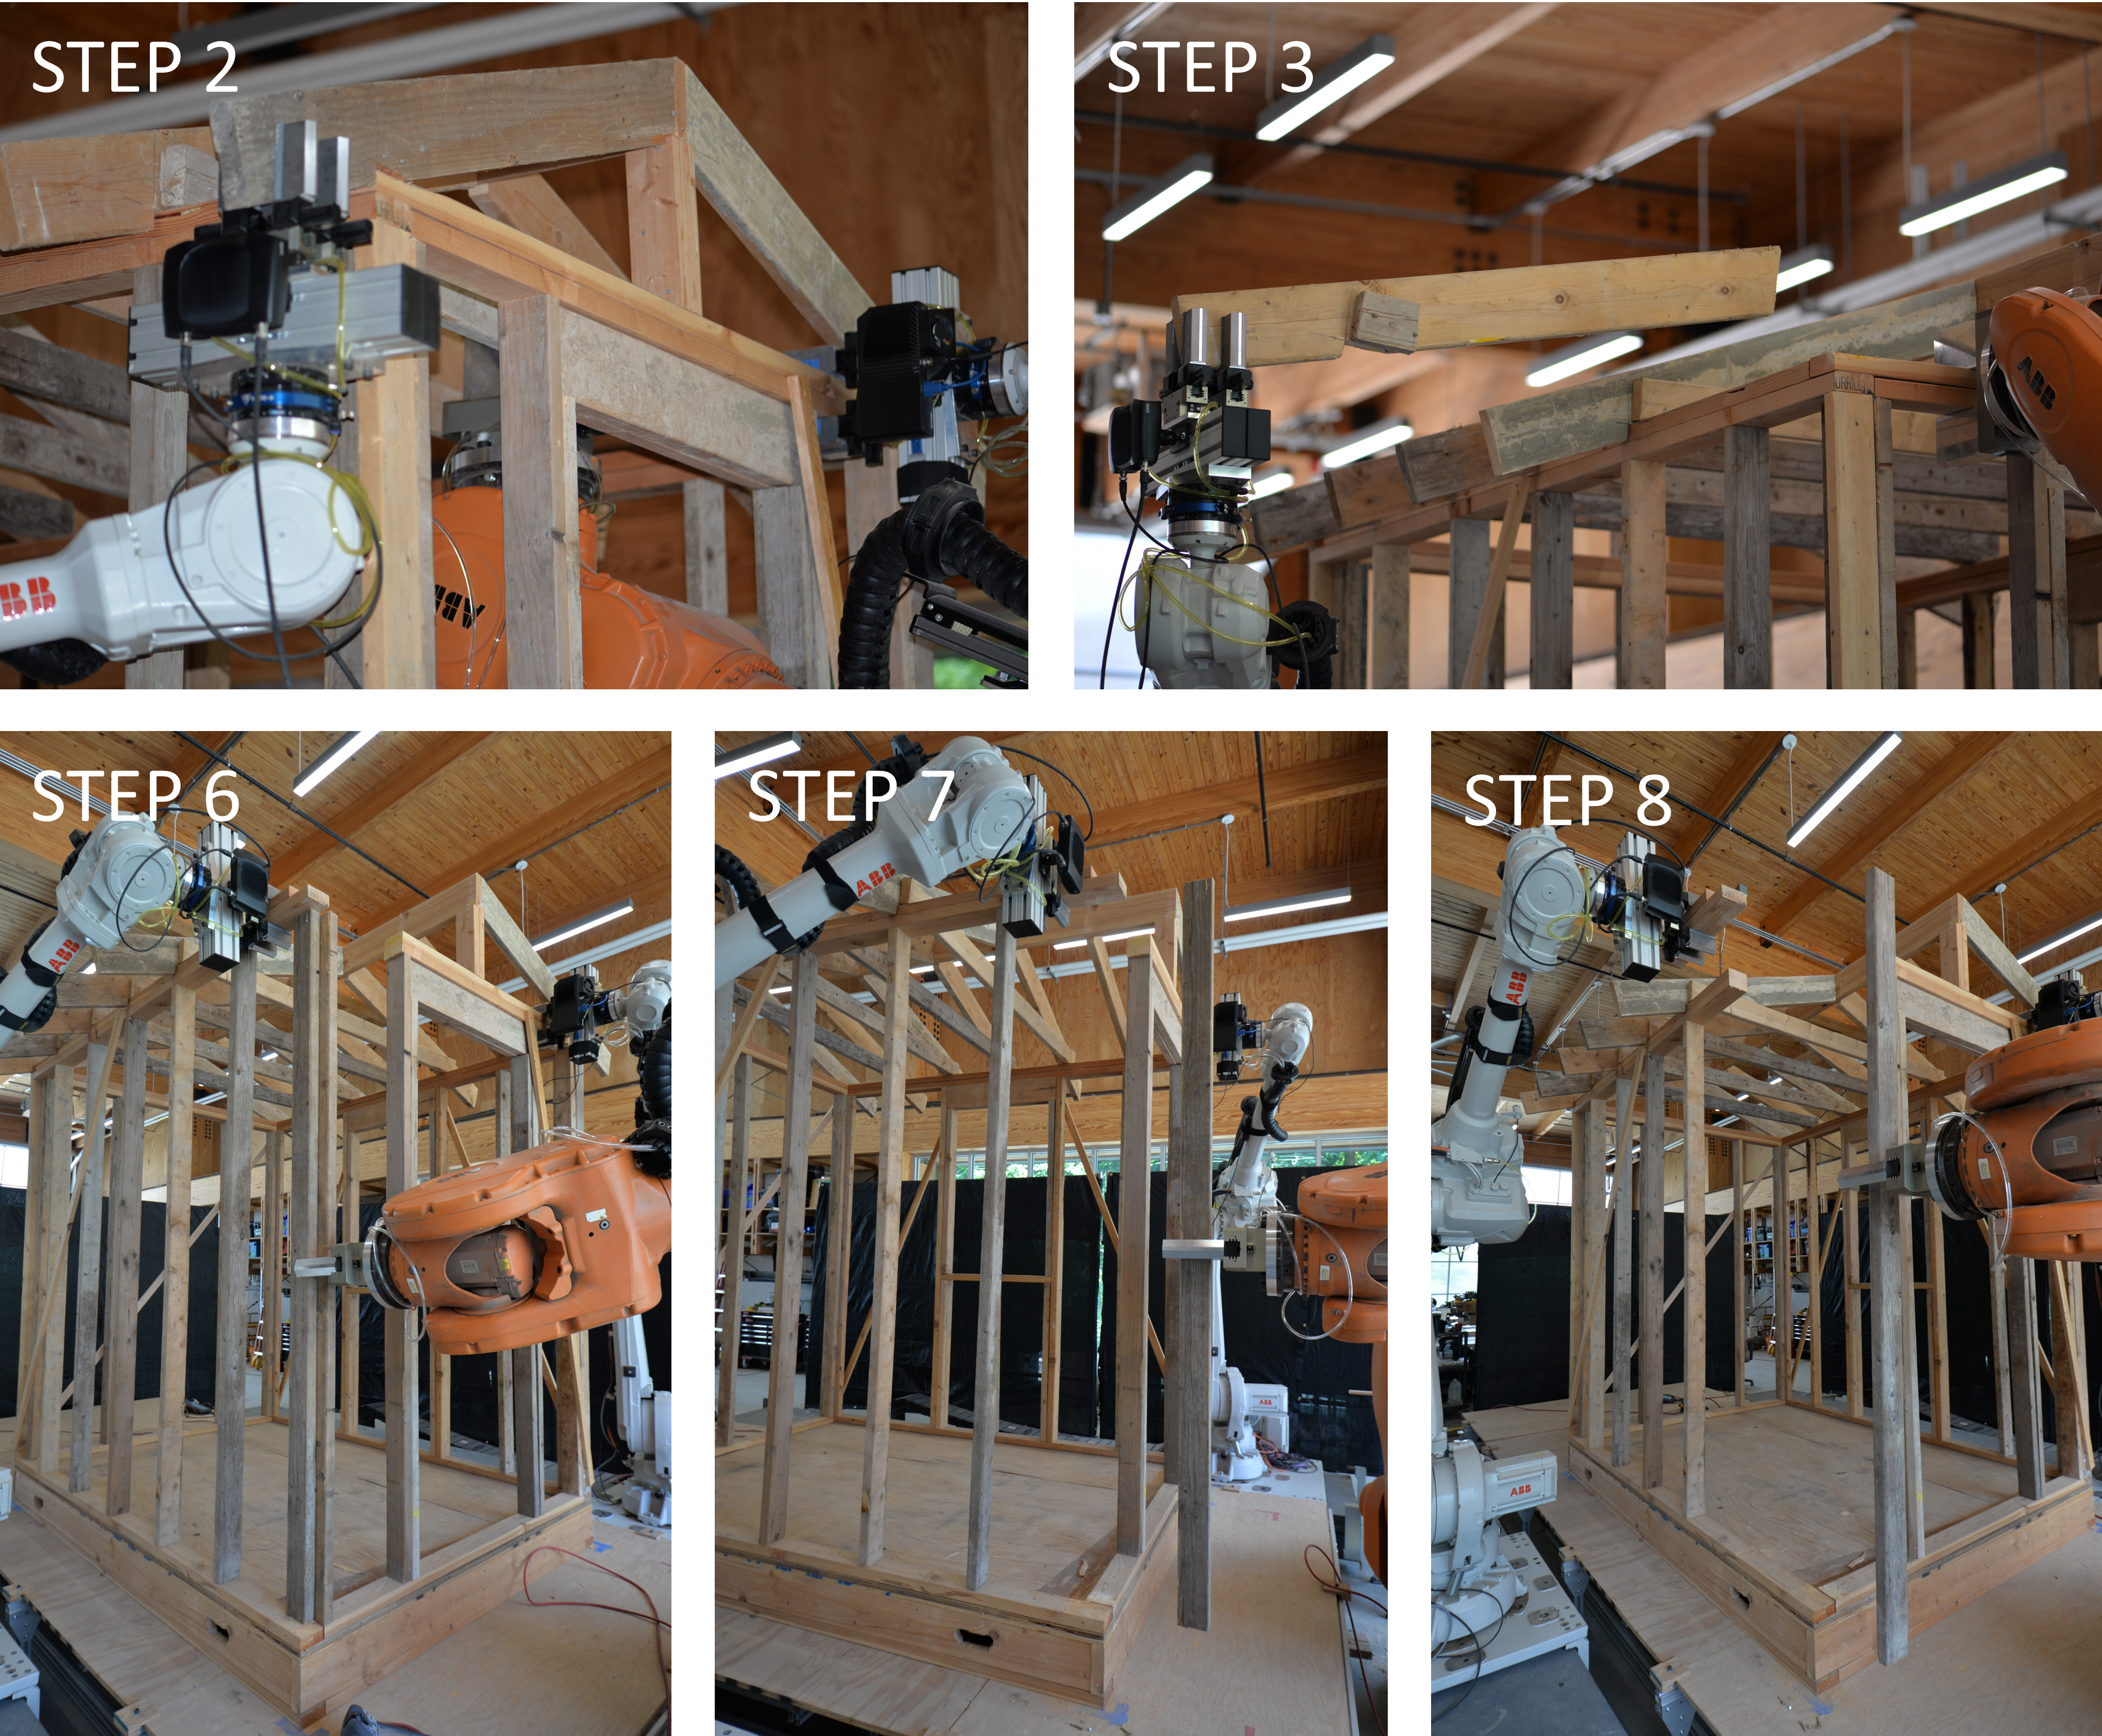
\includegraphics [trim={0cm 0cm 0cm 0cm}, clip, width=0.99\linewidth]{fig99_appendix_phase1_1}
        \caption{Phase 1 fabrication photos}
        \label{fig:fig99_p1_1} 
    \end{figure}

\clearpage
\subsection{Phase 2}\label{sec:appendixb_2}
    
    \begin{figure}[ht]
        \centering
        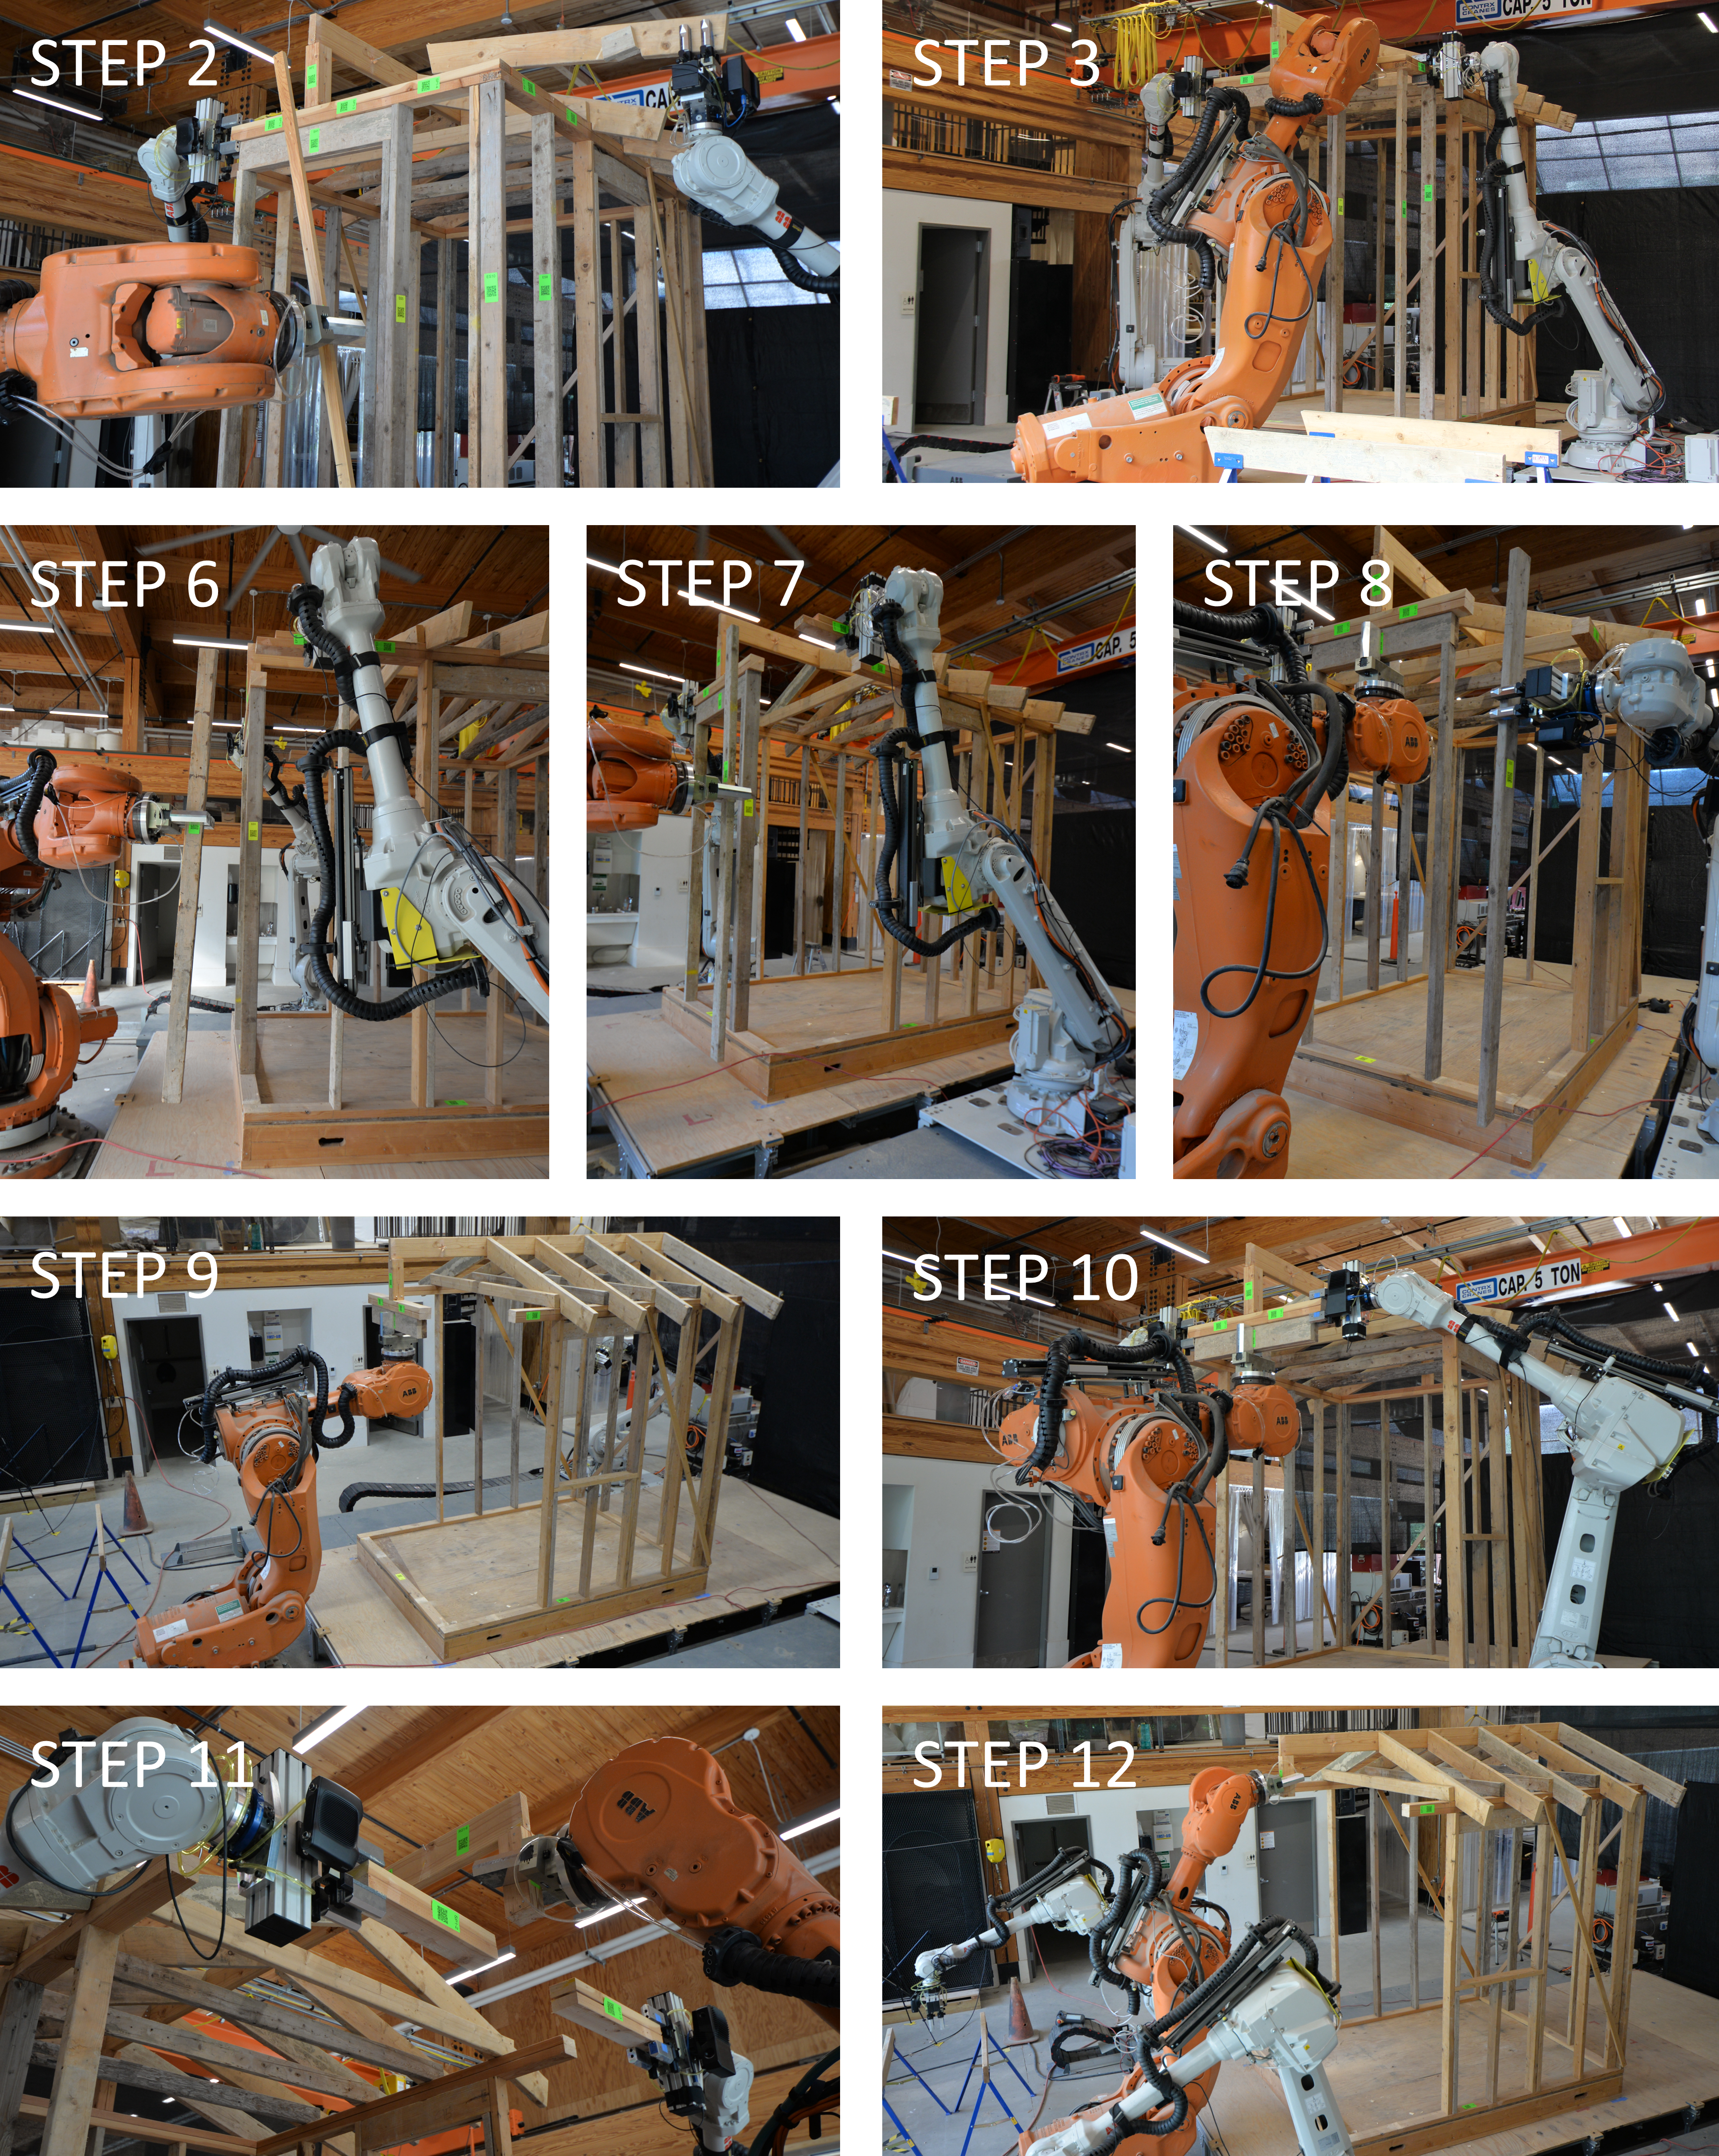
\includegraphics [trim={0cm 0cm 0cm 0cm}, clip, width=0.80\linewidth]{fig99_appendix_phase2_1}
        \caption{Phase 2 fabrication photos (disassembly)}
        \label{fig:fig99_p2_1} 
    \end{figure}

    \clearpage
    \begin{figure}[ht]
        \centering
        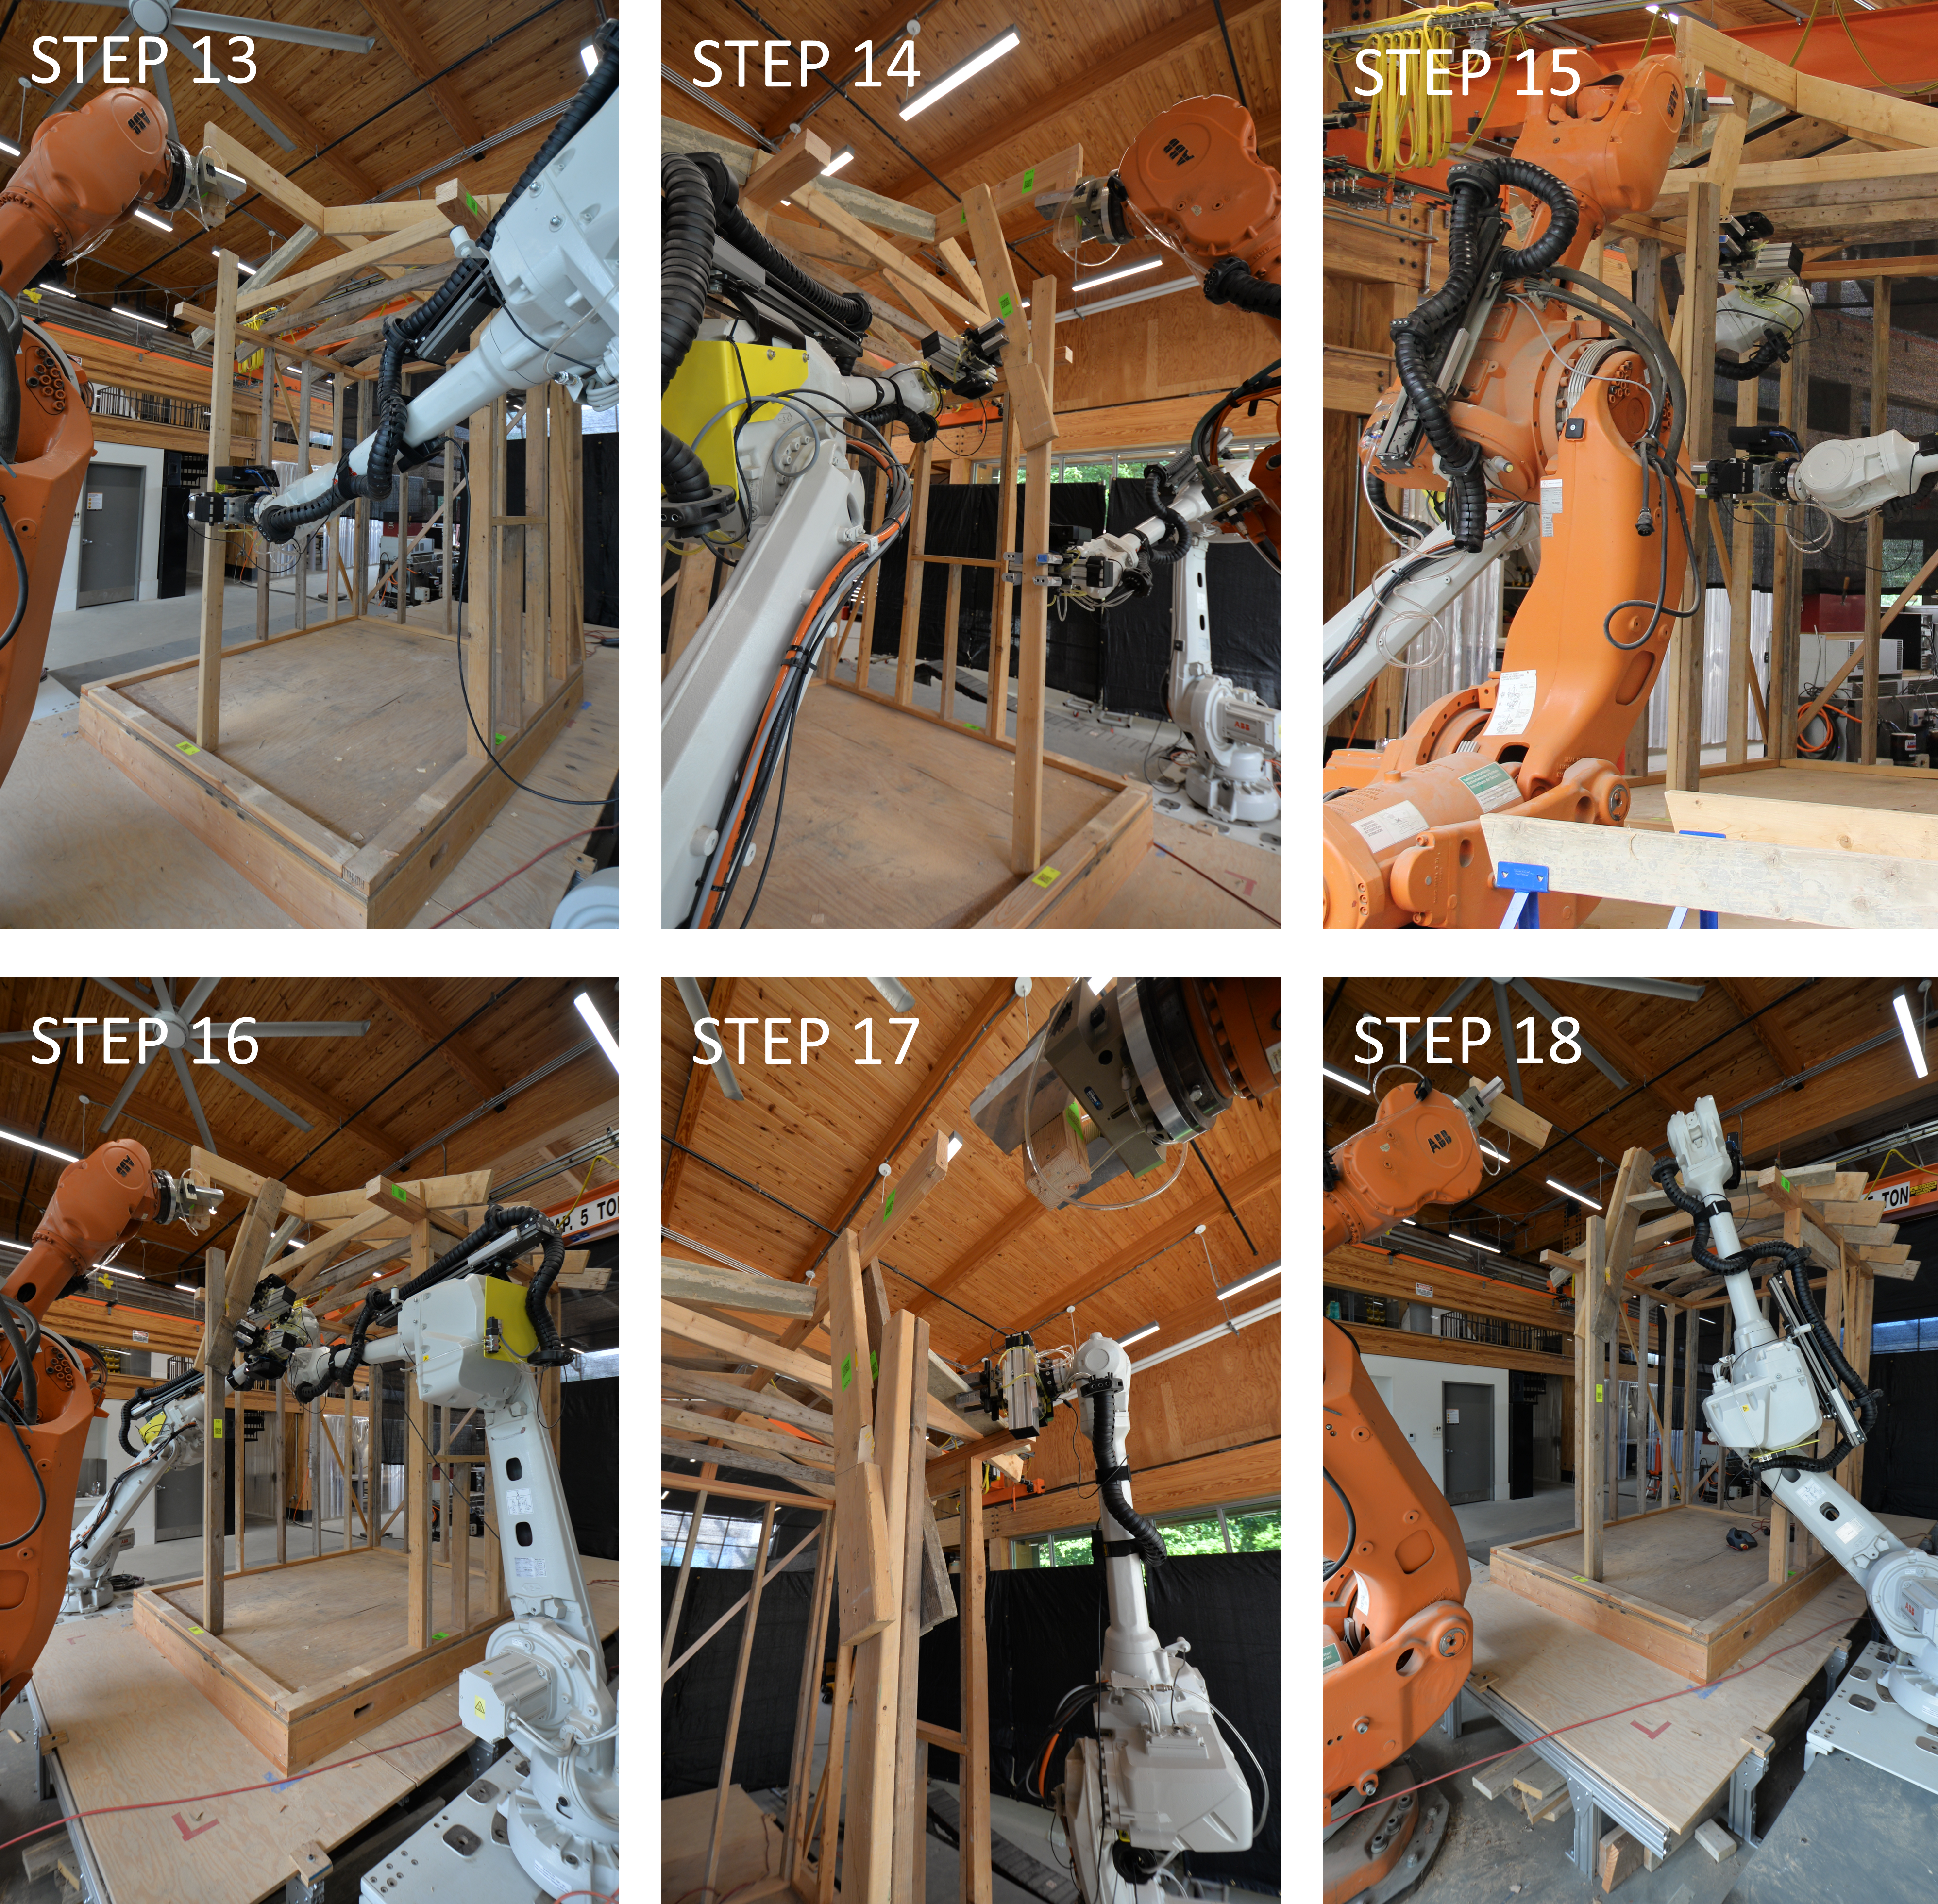
\includegraphics [trim={0cm 0cm 0cm 0cm}, clip, width=0.80\linewidth]{fig99_appendix_phase2_2}
        \caption{Phase 2 fabrication photos (reassembly)}
        \label{fig:fig99_p2_2} 
    \end{figure}


\clearpage
\subsection{Phase 3}\label{sec:appendixb_3}
    % \begin{figure}[h]
    %     \centering
    %     \includegraphics [trim={0cm 0cm 0cm 0cm}, clip, width=0.99\linewidth]{fig99_appendix_phase3_1}
    %     \caption{Phase 3 subgraphs corresponding to steps in sequence}
    %     \label{fig:fig99_p3_1} 
    % \end{figure}

    \begin{figure}[ht]
        \centering
        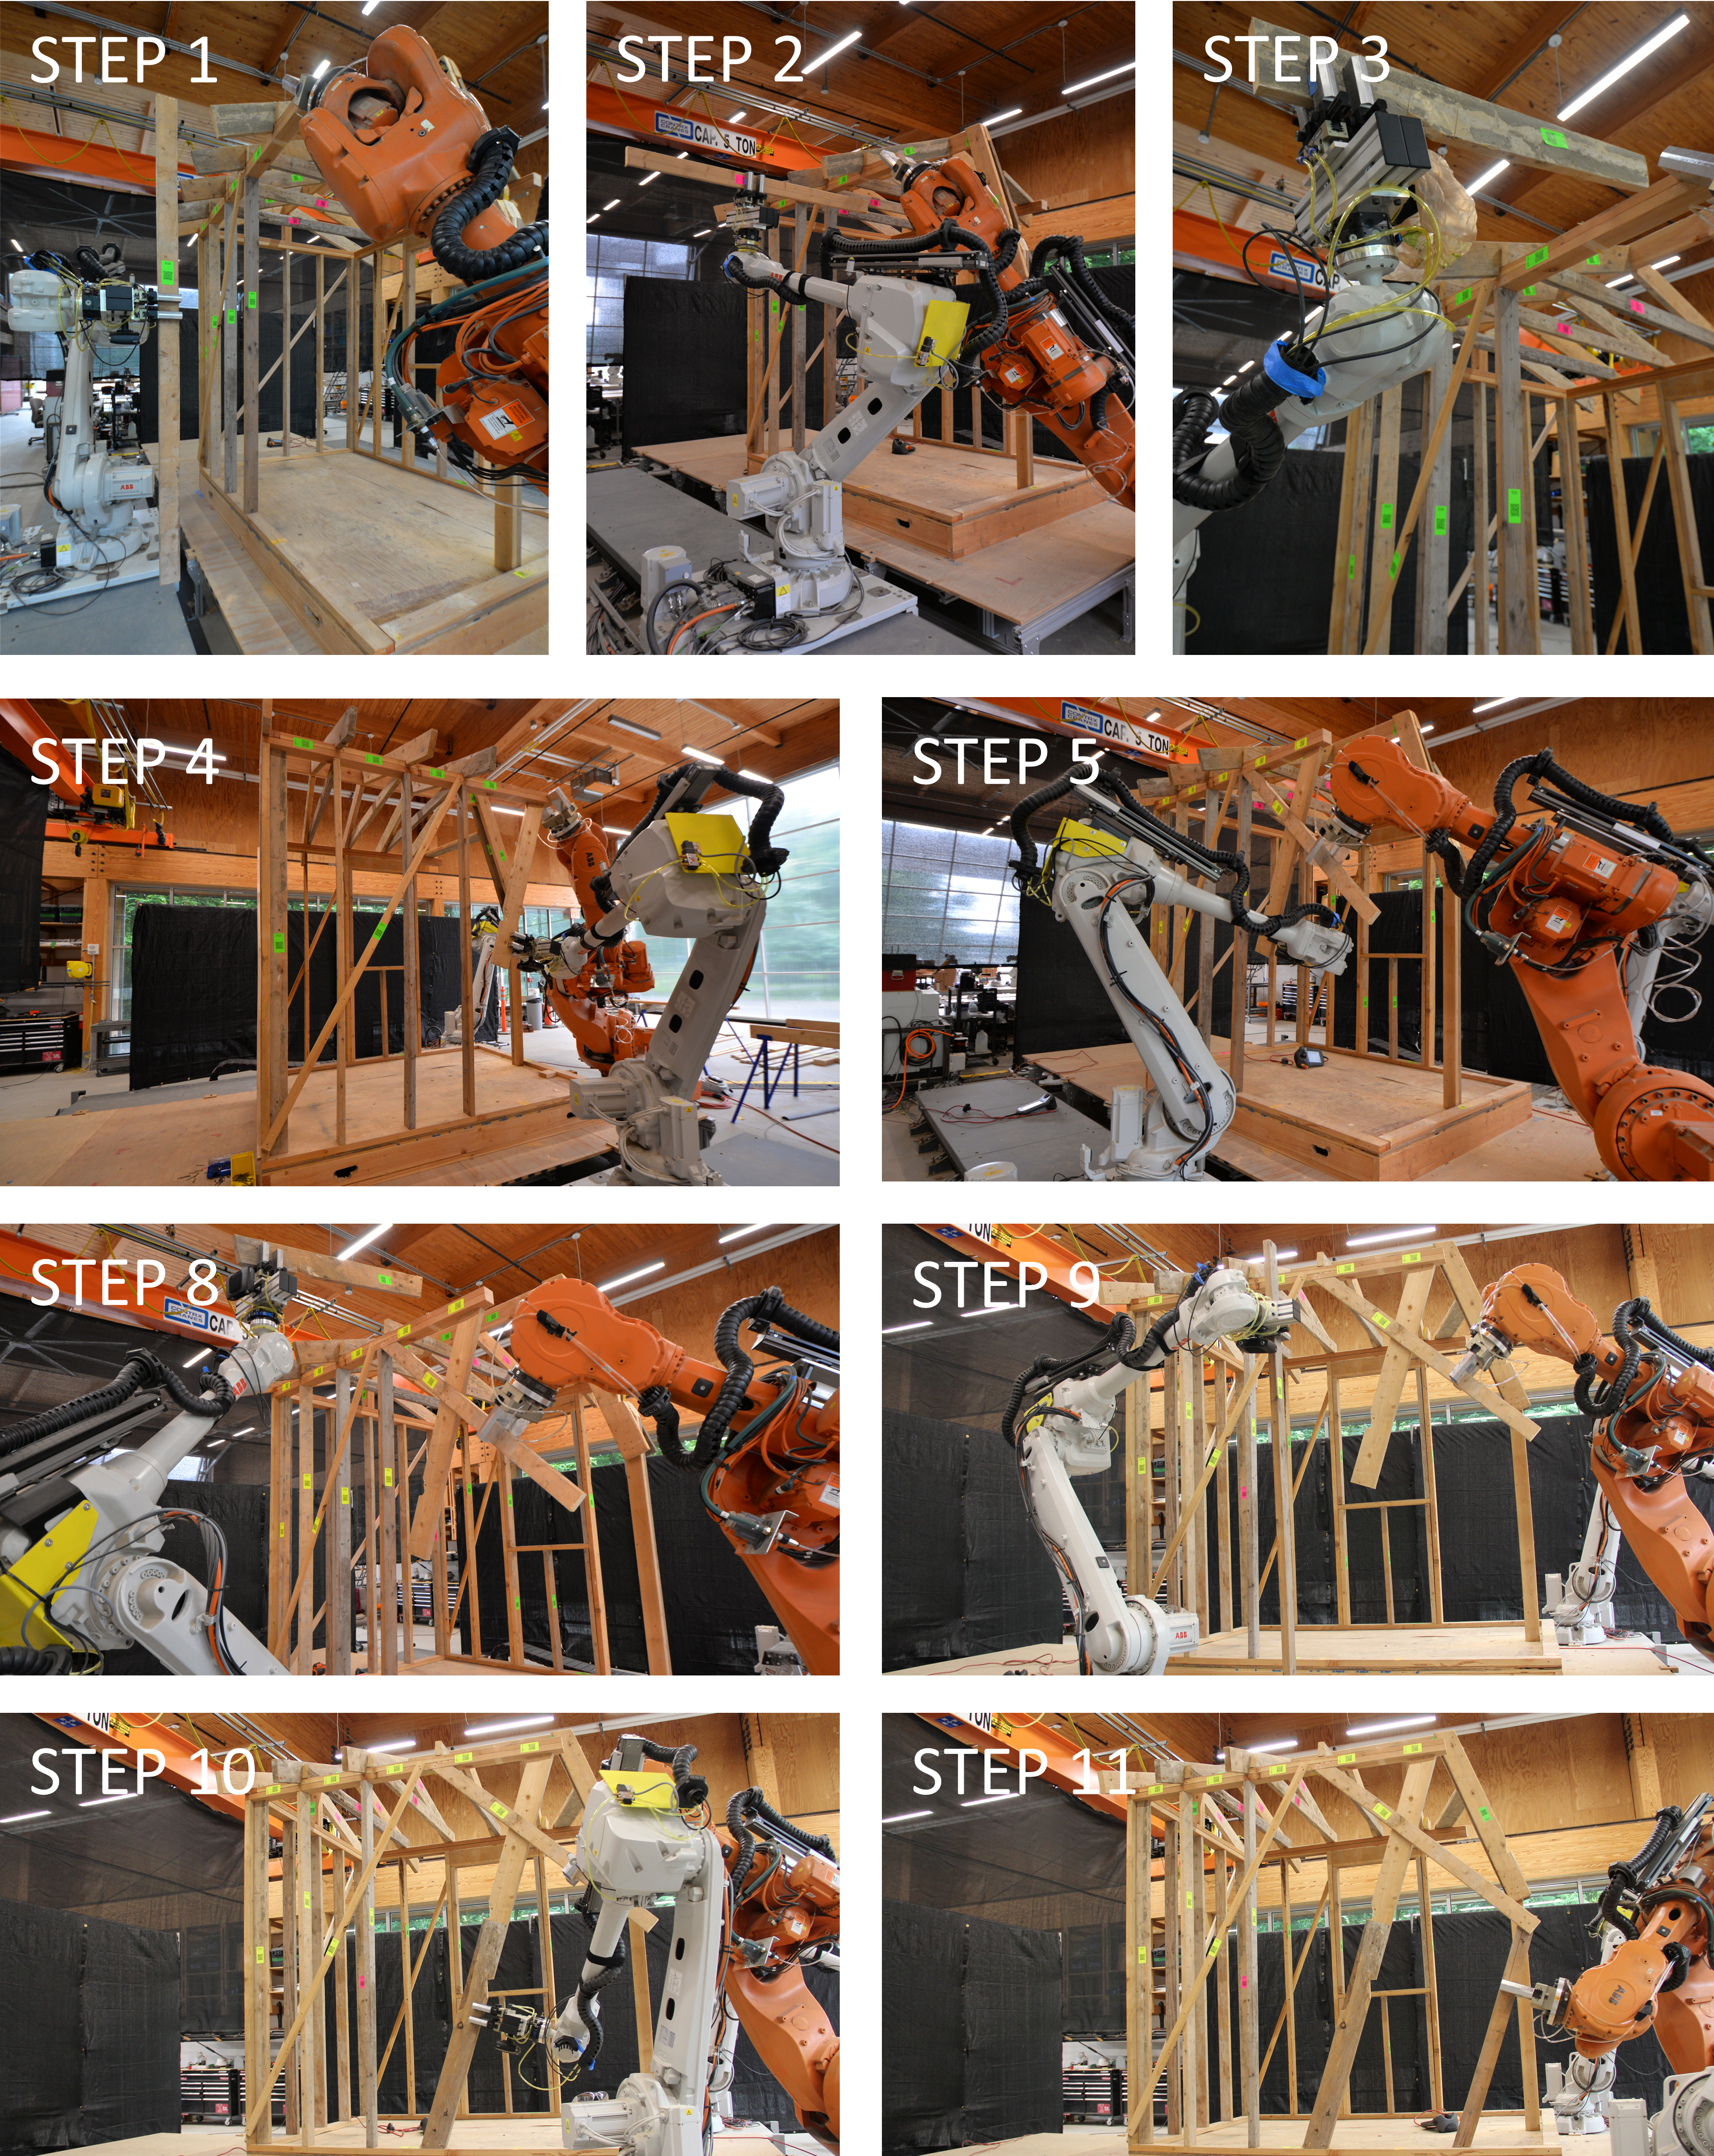
\includegraphics [trim={0cm 0cm 0cm 0cm}, clip, width=0.80\linewidth]{fig99_appendix_phase3_2}
        \caption{Phase 3 first half of disassembly/reassembly photos}
        \label{fig:fig99_p3_2} 
    \end{figure}

    \begin{figure}[ht]
        \centering
        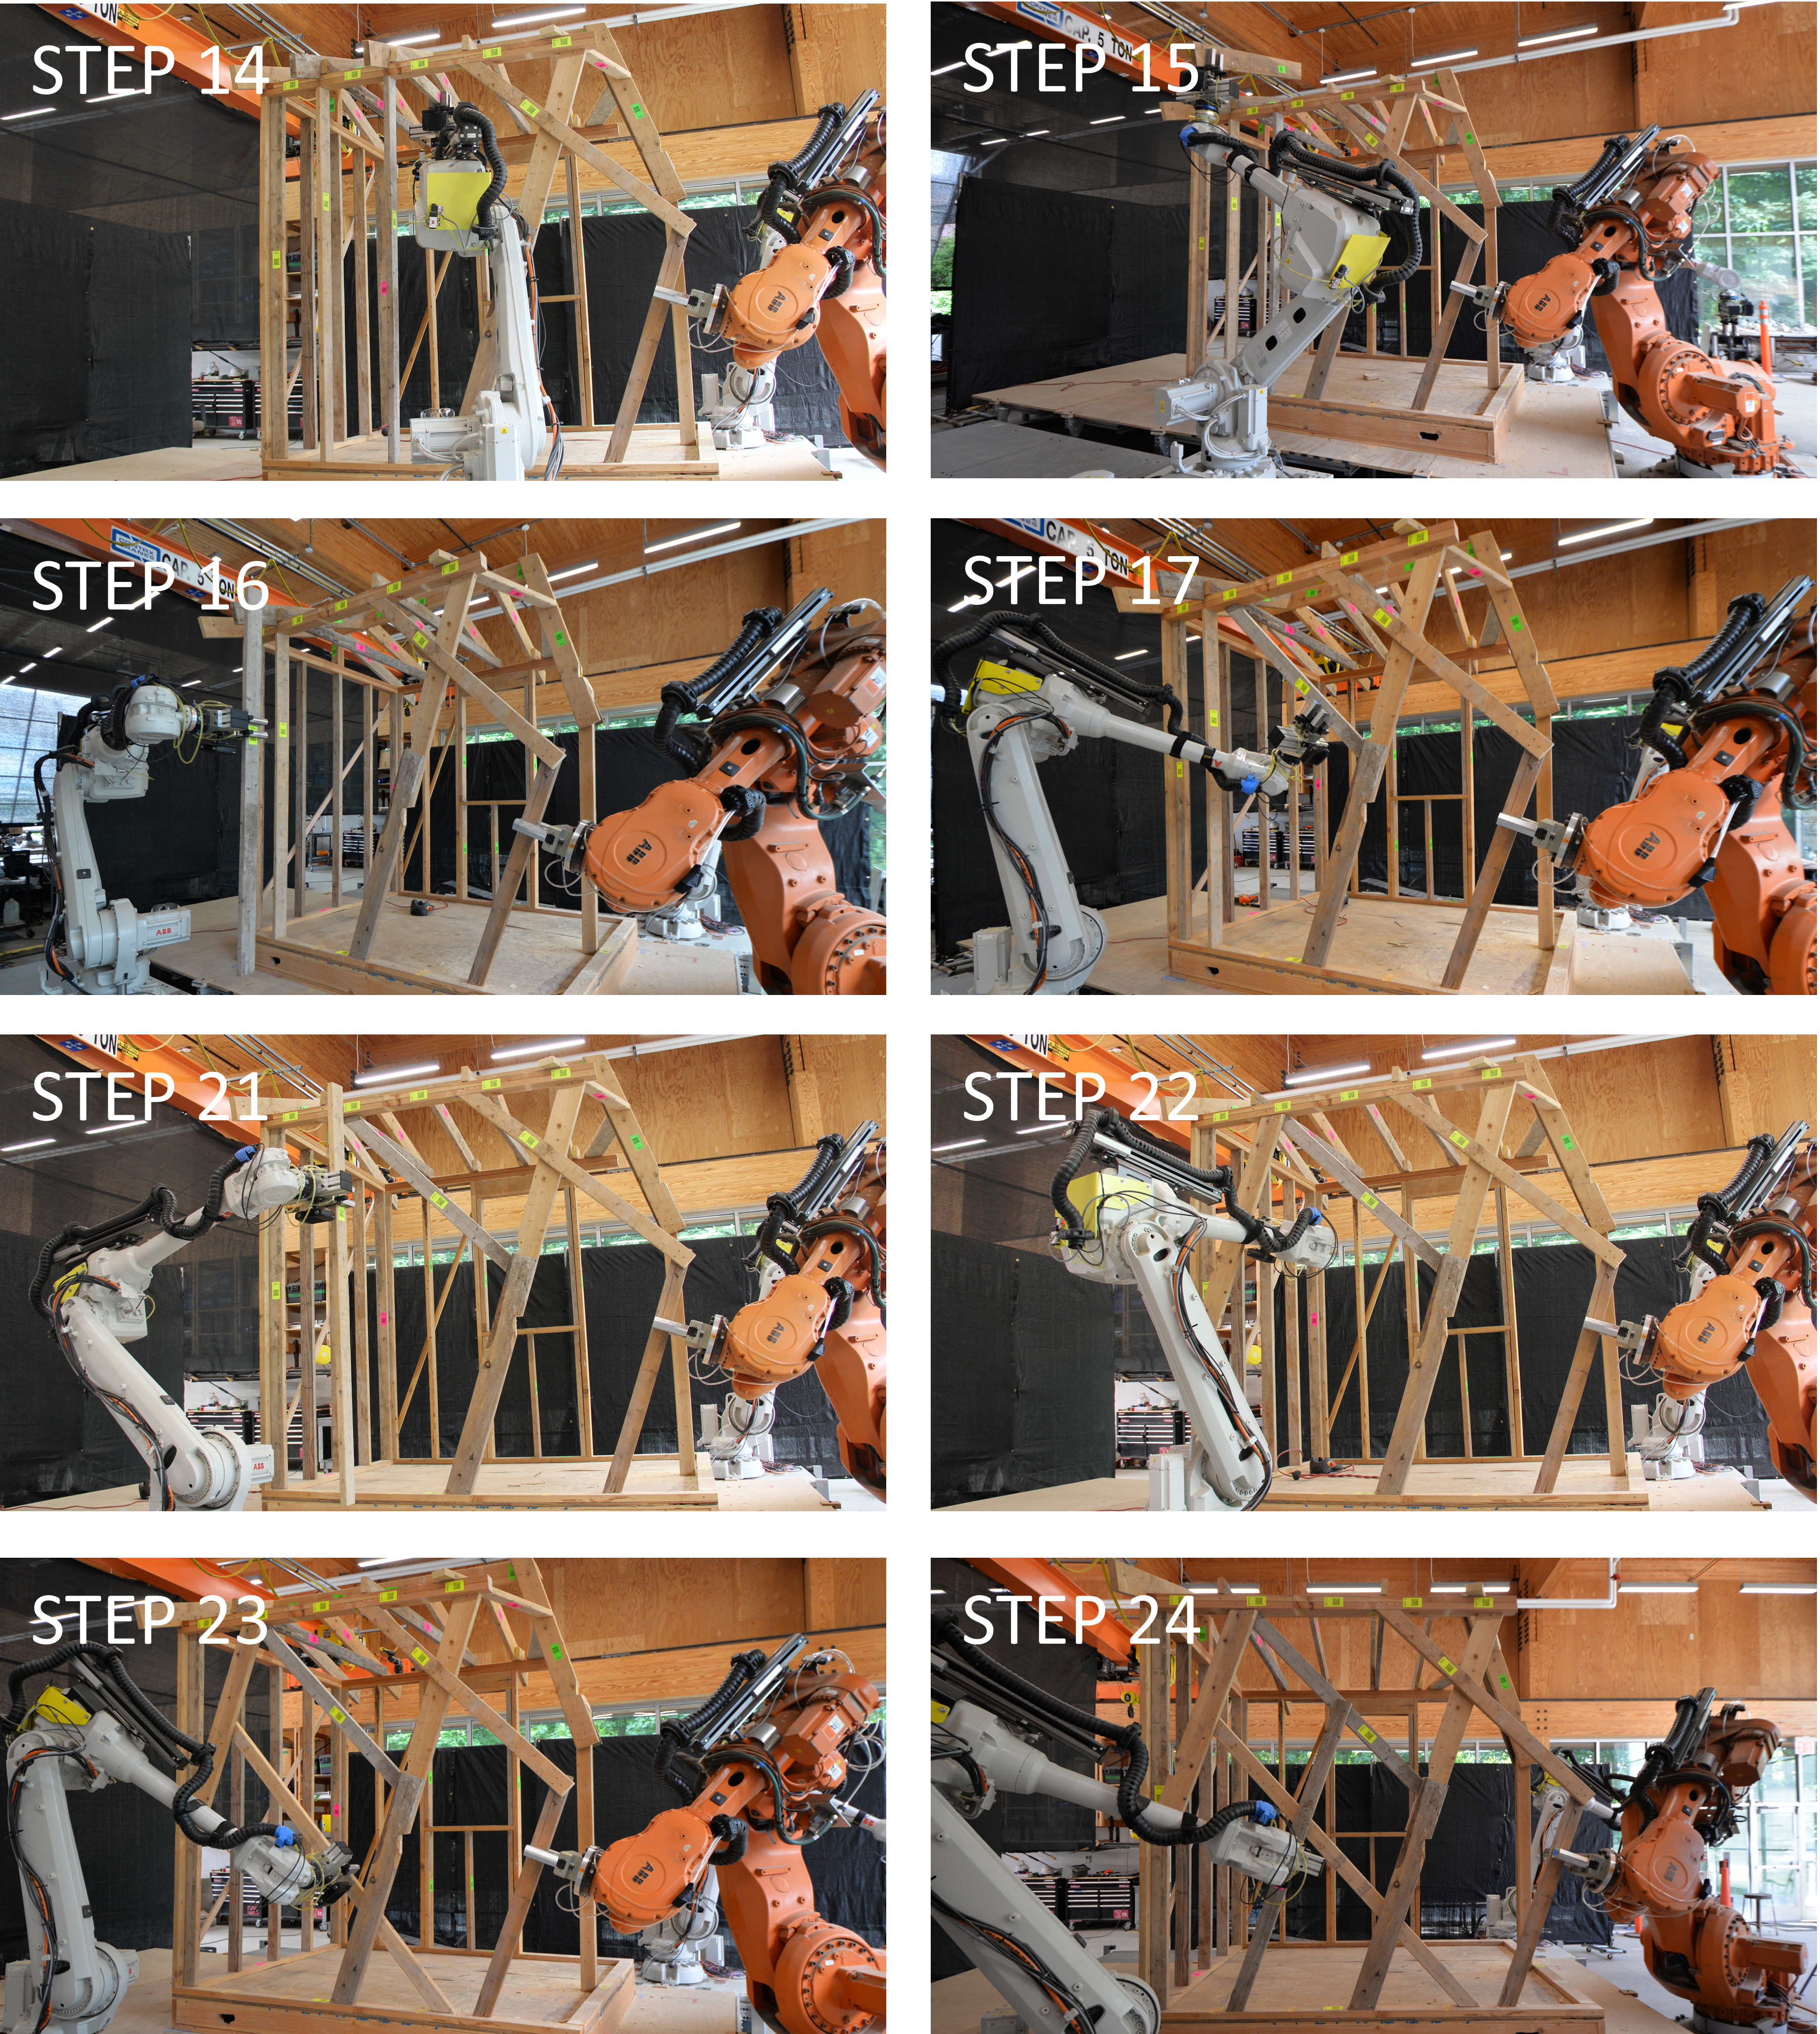
\includegraphics [trim={0cm 0cm 0cm 0cm}, clip, width=0.80\linewidth]{fig99_appendix_phase3_3}
        \caption{Phase 3 second half of disassembly/reassembly photos}
        \label{fig:fig99_p3_3} 
    \end{figure}

